\chapter{Background}

\section{Paraplegia and Rehabilitation}
Paraplegia is a medical term used to define where a patient loses feeling and/or movement in their lower two limbs. In comparison, quadriplegia (also sometimes known as tetraplegia) is the loss of control in all four limbs. It is important to note that not all feeling/movement needs to be lost in order for someone to be considered paraplegic \cite{IncompleteTraumaticQuadrilegia}. Only 30\% of all paraplegic and quadriplegic patients are considered complete lesions, where there is no sensation and no mobility in the lower limbs \cite{RehabParaplegia}. 

\begin{figure} [ht!]
    \centering
    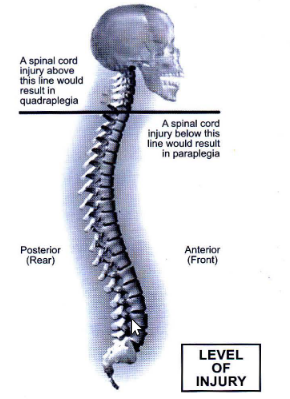
\includegraphics[width=0.5\linewidth]{Figures/Background/ParaQuadInjuryLocs.png}
    \caption{Location of spinal cord injury will determine type of paralysis \cite{RehabParaplegia}}
    \label{fig:ParalysisLocation}
\end{figure}

Paralysis is usually caused by trauma, such as sports injuries, vehicle accidents, or accidental falls, when the spine gets injured (see \autoref{fig:ParalysisLocation}). However, it can also be caused by specific diseases, including multiple sclerosis, amyotrophic lateral sclerosis, stroke, and in specific cases cancer \cite{CausesParaplegia}. Common effects of paraplegia include:
 
\begin{itemize}
    \item Loss of mobility, reflexes, and sensation
    \item Muscular weakness and atrophy
    \item Hormonal variations
    \item Gastrointestinal and bowel/bladder problems
    \item Muscle spasms
    \item Reduced cardiorespiratory fitness and increased likelihood of cardiorespiratory issues
\end{itemize}

Paraplegic and quadriplegic patients also have a higher likelihood of developing skin complications due to their limited mobility and feeling. The limited feeling make skin complications more dangerous, while reduced blood flow to affected limbs increase the recovery time of any dermatological issues \cite{SPISecondaryEffects}. Pressure ulcers are a common example of skin complications in patients suffering from spinal cord injuries, with those suffering from higher levels of paralysis at a higher risk. In fact, a study \cite{PressureUlcerRiskParalysis} discovered that 1/3 of its subjects suffered from at least 1 pressure ulcer in both pre-study analysis as well as throughout the four stages of its study. Therefore, any device to be used with paralysis patients must more-so consider the safety and comfort of the patient.

Rehabilitation can play a key role in reducing these side effects in patients who experience paraplegia. Mainly, physical therapy for paralysis patients focus on three main types of exercises: stretching, strengthening, and aerobic. Additionally, paralysis patients may go through gait training with the assistance of medical devices.

\subsection{Physical Therapy for Paralysis Patients}

\begin{figure}[ht!]
    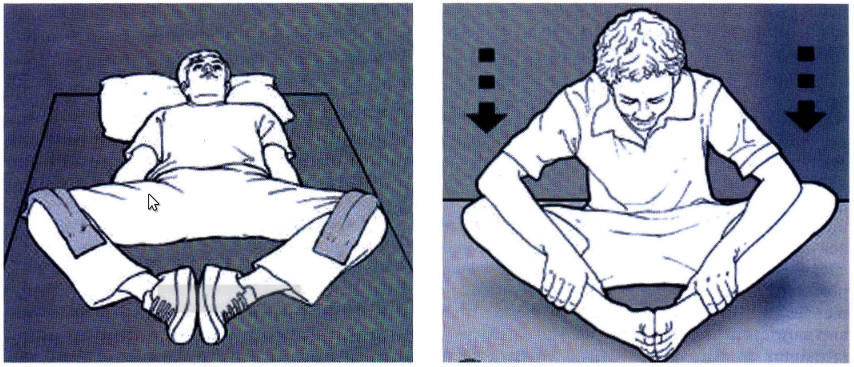
\includegraphics[width=\linewidth]{Figures/Background/BilateralAdductorStretch.png}
    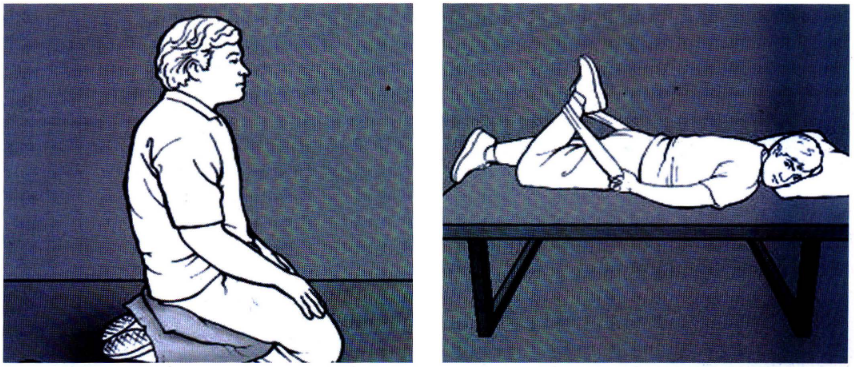
\includegraphics[width=\linewidth]{Figures/Background/QuadricepsStretch.png}
    \caption{Bilateral Adductor Stretches (top) and Quadriceps Stretches (bottom) for paraplegic and quadriplegic patients \cite{RehabParaplegia}}
    \label{fig:ParaplegiaStretches}
\end{figure}

\subsubsection{Stretching}
Stretching is considered one of the most important exercises \cite{RehabParaplegia}, more-so than any other form of exercise because it can be done often and at home. Carefully designed exercises (like seen in \autoref{fig:ParaplegiaStretches}) can improve flexibility, reduce muscle spasms, reduce the chance of injury, and relieve contractures \cite{ParalysisStretchingWeightLoadingPMID} \cite{ParalysisStretchingHarvey} \cite{ParalysisStretchingMichigan}. Some common stretches include bilateral adductor stretches, quadriceps stretches, and hip flexor stretches.

\subsubsection{Cardiorespiratory and Cardiovascular Training}
Due to the difficulty of exercise, cardiovascular and cardiorespiratory activities are also very important to maintain health in paralysis patients. Aerobic exercises can increase energy levels, improve lung and heart function, control body weight, and reduce fatigue \cite{RehabParaplegia} \cite{AerobicCapacityParaplegia}. A study showed that patients who suffer from neuromuscular deficiencies such as paraplegia suffered decreasing VO\textsubscript{2}max \footnote{VO\textsubscript{2}max is a common metric that measures the maximum rate of oxygen utilization during heavy exercise.} compared to control subjects with no issues \cite{AerobicCapacityParaplegia}. The combination of the upper and lower body exercise in paraplegic patients can strengthen the paralyzed limbs while also activating healthy limbs, and ultimately improve the overall health of the patient. Some researchers have even proposed introducing wheelchair racing as a sport in an effort to help with rehabilitation after paraplegia \cite{WheelchairRacingParaplegia}.

\subsubsection{Strength Training}
Improving strength in muscles may actually partially reverse the loss of mobility in partially paralyzed patients, while also improving muscle tone \cite{AerobicCapacityParaplegia} and preventing bone atrophy \cite{ParalysisStretchingWeightLoadingPMID}. This type of exercise can be split into two major regions: training of affected limbs and muscles, and the training of non-affected regions. Affected limbs can benefit from an increase in mobility and definition, and can generally reduce the likelihood of muscular atrophy. Additionally, strong hip and leg muscles in partially paraplegic patients can help in gait training and increase the possibility of usage in life. On the other side, increasing or maintaining strength in unaffected regions can help with quality of life improvement. Often, paraplegic patients may elect to use crutches or canes as an assisted mobility device in the real world. Increasing arm/shoulder strength and endurance will also increase capability for patients to use some of these assisted devices. Finally, back and abdomen muscles are very important to strengthen to maintain posture and improve gait performance \cite{TrunkMuscleLoadingParaplegia}. 

\subsubsection{Hydrotherapy}
Hydrotherapy (exercising in water) is a notable way for patients suffering from paraplegia to better strengthen muscles and improve cardiovascular health. Due to similar buoyancy, water can reduce the effects of gravity without any external assistive devices. At the same time, the increased density of the water (in comparison to air) creates a natural resistance without the use of weights or elastics. Therefore, hydrotherapy is used in paraplegic patients to increase muscle power, increase endurance, and even help with gait training (see \autoref{sec:GaitTraining}). In minor cases of paralysis, some patients even use swimming as a way to exercise \cite{RehabParaplegia} \cite{BenefitsOfHydrotherapy}.

\subsection{Gait Training}
\label{sec:GaitTraining}

Gait training has become the best way to improve motor functions in those who have partially or fully lost mobility in their legs and torso. The premise of this exercise is to have patients do similar movements to what one would do without their disability, like walking and climbing stairs. Essentially, the goal is to help the patient relearn the gaits they previously knew. Spinal neuronal circuits degrade quickly - in just a year, they can lose most of their potency, essentially unlearning any gait abilities the patient had in the past \cite{GaitTrainingClinical} \cite{RehabParaplegia} \cite{TrunkMuscleLoadingParaplegia}. Gait training can help reconnect the broken spinal neurons, and improve motor function and balance in a patient. In fact, several studies have show that some patients with full spinal cord injuries have been able to recover part or even all of their walking capabilities through gait training \cite{GaitTrainingClinical} \cite{ImprovingGaitAdaptabilityInPatients}! 
\footnote{There is significant research in the benefits of gait training for paraplegic and quadriplegic patients. Not all prior work is cited here.} 

\subsubsection{Use of Assistive Devices for Gait Training}
Since most patients suffering from paralysis won't be able to hold themselves up, there have been many different proposals to compensate for gravity. At lower levels of paralysis, canes, walkers, and other walking assisted devices can help. Hydrotherapy has also been used with gait training due to the similar densities of humans and water \cite{BenefitsOfHydrotherapy}. With more serious cases of paralysis, robotic solutions and other active orthoses have been proposed and used in clinical settings.

Standard solutions like canes and walkers will only work for patients with mild paralysis. Canes are designed to support only 25\% of body weight \cite{RehabParaplegia}. They can also be fairly unstable, since they usually only have at most 4 points of contact with a very small ground contact area. Walkers are better than canes, since they can support up to 50\% of body weight \cite{RehabParaplegia}. However, canes, walkers, and crutches have one downside: the required upper-body strength. Mild lower-limb paralysis cases usually can benefit from these inexpensive tools to help with gait training. However most patients will struggle holding themselves up during gait training.

\begin{figure} [ht!]
    \centering
    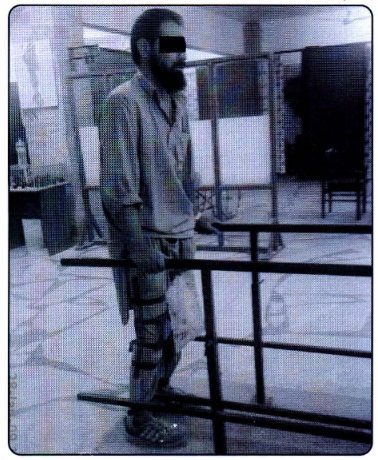
\includegraphics[width=0.4\linewidth]{Figures/Background/SplintsDemo.png}
    \caption{Patient using basic splint orthosis \cite{RehabParaplegia}}
    \label{fig:SplintsDemo}
\end{figure}

Orthoses are the next level up in assistive devices. They can come in many different shapes and can be designed to fit a patient's progress. At the lowest levels are specialty splints or braces (seen in \autoref{fig:SplintsDemo}) that can help keep joints locked or reduce load of a joint through passive springs. These solutions often cost very little in material, and apply normal loads on the user's skeletal system - helping to prevent bone atrophy. Actively powered orthoses also exist with various levels of research and clinical trials (see \autoref{sec:OtherExos}), and can be separated in two major groups. 

\begin{figure}[ht!]
    \centering
    \includegraphics[width=0.4\linewidth]{Figures/Background/OtherExos/LARRE_old.png}
    \hspace*{10mm}
    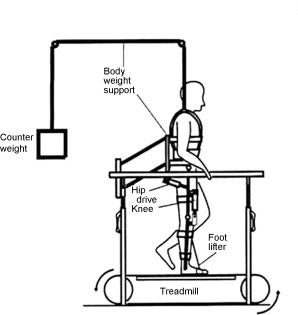
\includegraphics[width=0.4\textwidth]{Figures/Background/ExoSeparateGravityComp.png}
    \caption{Comparison between an exoskeleton with active gravity compensation (left) and an exoskeleton with passive gravity compensation (right) \cite{GaitTrainingClinical}}
    \label{fig:ExoTypesGCSCompared}
\end{figure}

Actively compensating exoskeletons, as shown in the left image in \autoref{fig:ExoTypesGCSCompared}, are orthotic devices that use various types of actuators, sensors, and gait controllers to help keep patients standing and walking with little to no strength required (from the patient). These types of exoskeletons use up a significant amount of energy, since they must essentially do all the physical work that leg muscles would normally do. This usually means powerful actuators and motors with precise and stable control, and large batteries (which add to overall weight) or a large/long tether. Such power increases the overall flexibility of the system, however, at a cost. It also increases complexity of the control software, and introduces a safety risk of attaching powerful actuators to patient limbs.

To mitigate some of these risks, some solutions separate the exoskeleton and the gravity compensation (see right image in \autoref{fig:ExoTypesGCSCompared}). A separate mechanical system supports the weight of the user usually through a counterweight system or a gantry of some sort. This allows for the actuator in the exoskeleton orthoses to be weaker or power (current) limited to prevent injury in case of a malfunction. However, such systems are much more limited in their uses, since the power is hardware limited and more infrastructure is needed to use the device. Additionally, any actively compensating exoskeleton orthoses can be current limited and be used with a mechanical gravity compensation system. 

However, one of the biggest struggles with orthoses is the dermatological problems that they may cause if the orthosis does not match the user's natural bone and skin movement. As explained earlier, patients suffering from paralysis are at an increased risk of developing skin complications \cite{DermatologicalIssuesParalysis}. This can be at least partially attributed to reduced sensitivity in paralyzed areas of the body. Therefore, any assisted devices that attach to a patient's skin should accurately follow the natural trajectory of the skin to avoid unnecessary rubbing.

\section{Human Knee Model}
\label{sec:KneeModel}

The human knee was initially considered as a pin joint, but research has suggested differently. A 1992 study using 5 subjects demonstrated that the joint does extend as it bends by attaching motion capture markers to the femur and tibia. It also suggested that there was a difference between loaded and unloaded knees \cite{3DKinKneeJointOldStabby}. 

\begin{figure}[ht!]
    \centering
    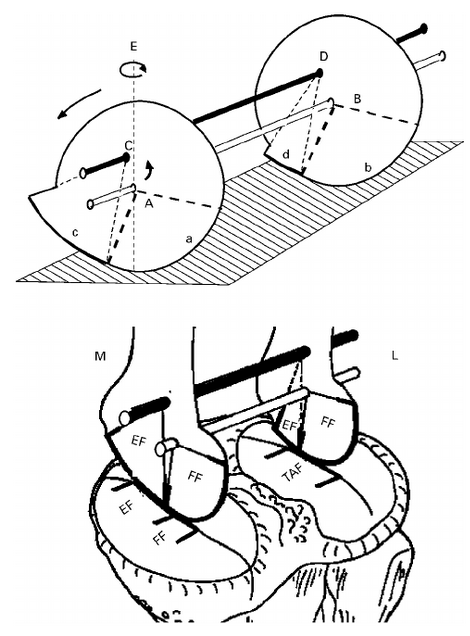
\includegraphics[width=0.5\textwidth]{Figures/Background/KneeAnatomy1.png}
    \caption{Diagram from \cite{MRIKneeShape_Unloaded} depicting the internal anatomy of a knee with respect to the movement patterns. The movement characteristics can be closely related to a cam mechanism}
    \label{fig:KneeAnatomyCam}
\end{figure}

Several studies since then have confirmed a non-linear knee flexion and extension relationship, as well as the difference between loaded and unloaded knees. Instead of intrusive motion capture markers, modern Magnetic Resonance Imaging (MRI) and advanced motion capture systems \cite{ModelAnalysisDeepKneeFlexion} has allowed for more precise bone tracking for both unweighted and weighted knee joints, since a 3 dimensional model can be built of the joint. A study performed by Iwaki \textit{et. al} using MRI data of cadaver knee joints found that the femur posterior circular arc is responsible for the linear extension of the leg through the flexion process, similar to the movement of a mechanical cam (see \autoref{fig:KneeAnatomyCam}) \cite{MRIKneeShape_Unloaded}. Through the bending process, the joint didn't rotate much outside the plane of flexion. These results were further confirmed during the dissection of the cadavers as well as in the followup research with live human knee joints \cite{MRIKneeShape_Loaded}. Additionally, the research also showed tibiofemoral motion changes by roughly 4mm when the knee joint was loaded.

\begin{figure}[ht!]
    \centering
    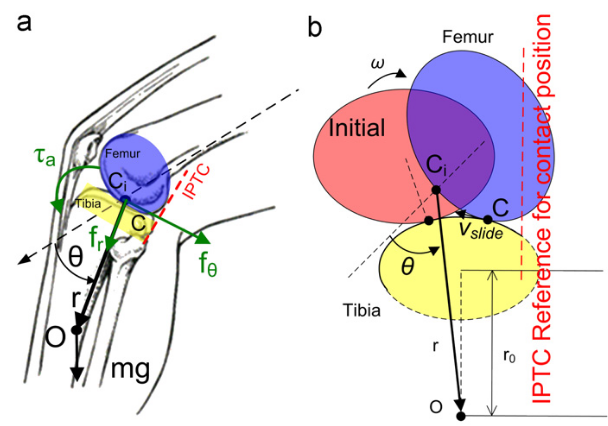
\includegraphics[width=0.8\textwidth]{Figures/Background/KneeParameterization.png}
    \caption{Diagram showing knee rotation \cite{KinDynKneeJoint}: (a) demonstrates the tibia's rotation around an initial contact point \(C_i\). (b) shows the femur and tibia relationship using parameterized shapes between the distance \(r\) and flexion angle \(\theta\)}
    \label{fig:KneeParameterization}
\end{figure}

This research was taken a step further with the parameterization of a knee joint's flexion and extension. The goal was to define a knee joint model to better create artificial mechanisms for rehabilitation exoskeletons. Based on MRI data of unloaded knees from \cite{MRIKneeShape_Unloaded}, ellipses were fitted to the ends of the tibia and femur to approximate the relationship between the distance \(r\) and flexion angle \(\theta\). The resultant tibia to femur relationship can be seen in \autoref{eq:TibiofemoralRelationship} and \autoref{fig:KneeFlexionCurve} \cite{KinDynKneeJoint}.

\begin{equation}
    r(\theta) mm = 1.078\theta^4 - 11.184\theta^3 + 26.524\theta^2 - 0.825\theta
    \label{eq:TibiofemoralRelationship}
\end{equation}

\begin{figure}[ht!]
    \centering
    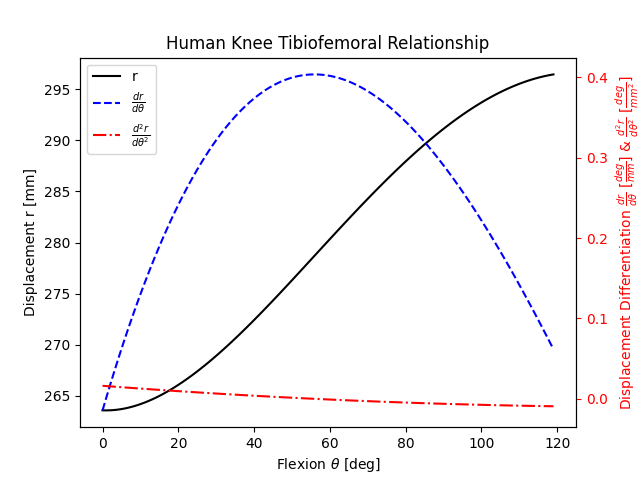
\includegraphics[width=0.9\textwidth]{Figures/Background/FlexionCurve.png}
    \caption{Relationship between tibia and femur during the flexion of the joint. \(r(m)\) is the distance between joint point of contact (\(C_i\) in \autoref{fig:KneeParameterization}) and center of mass of the tibia.}
    \label{fig:KneeFlexionCurve}
\end{figure}

These studies measure the relationship of the bones in the knee joints, and not the skin movement around the joint. However, exoskeleton orthoses are usually connected directly to the skin. In order for the research presented above to be applicable to orthoses, a relationship between the skin and femur/tibia must be made. A study by Benoit \textit{et. al} looked at 8 healthy males to compare the bone and skin movement in and around the knee joint in order to identify if skin markers are sufficient to determine bone kinematics around the knee. Each subject had intra-cortical bone-pins inserted in the proximal tibia and distal femur with 3 motion capture markers on each pin. Then, 8 total motion capture markers were attached directly to the skin to measure the difference in the movement (see \autoref{fig:SkinBoneRelationshipStudy}). 

\begin{figure}[ht!]
    \centering
    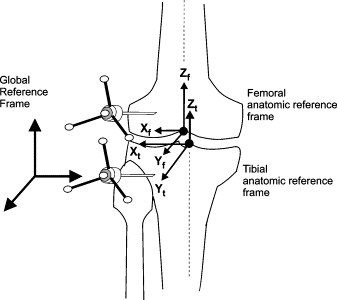
\includegraphics[width=0.6\linewidth]{Figures/Background/SkinMovementResearch_Diagram.jpg}
    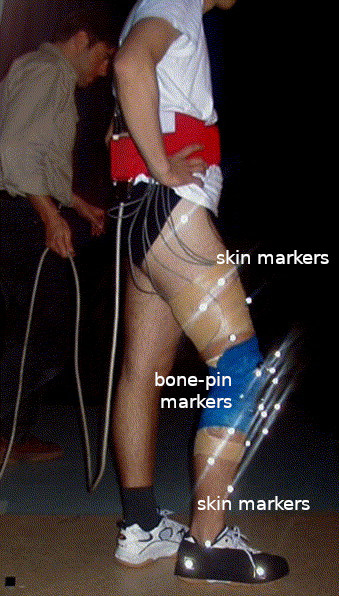
\includegraphics[width=0.3\linewidth]{Figures/Background/SkinMovementResearch_ImageMarked.jpg}
    \caption{Depiction of the research showing the relationship between skin and bone movement: (left) a figure illustrating the location of the bone-pins and (right) showing an image of a subject with all markers attached to them \cite{SkinMovementKneeKin}}
    \label{fig:SkinBoneRelationshipStudy}
\end{figure}

The results of this study seemed to show a significant difference between the skin and bone movement during several different gaits; average rotational errors were between \(4.4^\circ\) and \(13.1^\circ\) while translational errors averaged up to 16.1mm \cite{SkinMovementKneeKin}. What is more interesting is that the errors measured remained relatively constant between different movements, seemingly demonstrating that the error comes from the different connection methods (skin vs bone) and not via measurement tolerances. The researchers were able to conclude that skin-marker kinematics around the knee are not representative of the motion of the bone inside the knee joint. We may be able to therefore inversely conclude that bone kinematics may not be a good representation when designing knee orthoses. However, the research had a relatively small sample size due to the invasive nature of the experiment, and attached markers directly to taped up thighs (see \autoref{fig:SkinBoneRelationshipStudy}), which may have failed to represent the actual skin movement. Another similar study which looked at skin and bone movement in 3 individuals around the knee during running concluded with rotational errors of \(21\%\) for flexion/extension, \(63\%\) for internal/external rotation, and \(70\%\) for abduction/adduction. However, these results were highly subject dependent. Therefore, more research is needed to conclude the relationship between a skin connection on the thigh and a skin connection on the shank (calf) for the purpose of rehabilitation exoskeletons.

% Todo: [minor] if time, add a section on knee orthoses
% \subsection{Current Knee Orthoses}

\section{Exoskeleton Orthoses}
\label{sec:OtherExos}
Exoskeletons are an interesting application to help those with paralysis rehabilitate and exercise their muscles. They can take programmatically reduce or add bodyweight to the user to aid with safe gait training and muscle development. Additionally, powered exoskeletons can help move patient legs in the motion of a gait to help with relearning gait cycles such as walking and climbing stairs. The flexibility these rehabilitation devices offer have been noticed, and several different solutions exist at different levels of clinical implementation. Several studies have demonstrated clinical benefits to using exoskeletons for paralysis patients. \cite{ExoMobilityOutcome} suggested that people with partial paraplegia and tetraplegia were able to quickly learn how to walk with an exoskeleton on different surfaces. Users are able to walk up to \(0.55m/s\) after several weeks of training and practice, compared to an average walking speed of \(1.4m/s\) for ambulatory people \cite{IndigoClinicalStudy}. Studies have even demonstrated a clinically significant improvement in mobility \cite{GaitTrainingBenefitsRoboticsWalkbot} \cite{ImprovingGaitAdaptabilityInPatients} \cite{RoboticGaitTraining}; some complete paralysis patients using body weight supported gait training with exoskeletons and other rehabilitation devices have been able to regain most of their mobility back \cite{GaitTrainingClinical}!

\subsection{WPI LARRE}
\label{sec:larre}
\begin{figure}[ht!]
    \centering
    \includegraphics[width=0.7\linewidth]{Figures/Background/OtherExos/LARRE_old.png}
    \caption{The WPI LARRE rehabilitation exoskeleton \cite{SpringWrapClutchKnee}}
    \label{fig:LARRE_Background}
\end{figure}

The WPI LARRE (Legged Articulated Robotic Rehabilitation Exoskeleton) is an exoskeleton project developed by the \href{http://aimlabdev.wpi.edu} {Worcester Polytechnic Institute (WPI) Automated and Interventional Medicine (AiM) Lab}. The research presented in this thesis directly contributes to the AiM Lab's effort to develop an exoskeleton for rehabilitation of lower-limb paralysis patients. 

The project was originally started and named as the HEX Gen-1. It's goal was to help with studying rehabilitation of patients who have suffered from spinal cord injury using exoskeletons. The project also offers a platform to develop software and hardware technology for rehabilitation exoskeleton. Therefore, it is designed to be adaptable to research different control systems and joint types. The hip joint is powered by a brushless DC motor (Maxon EC90, Maxon Group), while the knee and ankle joints aren't actively powered by any motor. Instead, the knee joint contains a spring wrap clutch/brake to help provide support to patients throughout their gait cycles as proposed by \cite{SpringWrapClutchKnee}. Additionally, the ankle joint included a spring to add force during dorsiflexion to help in walking gaits.

\subsection{H2}

\begin{figure}[H]
    \centering
    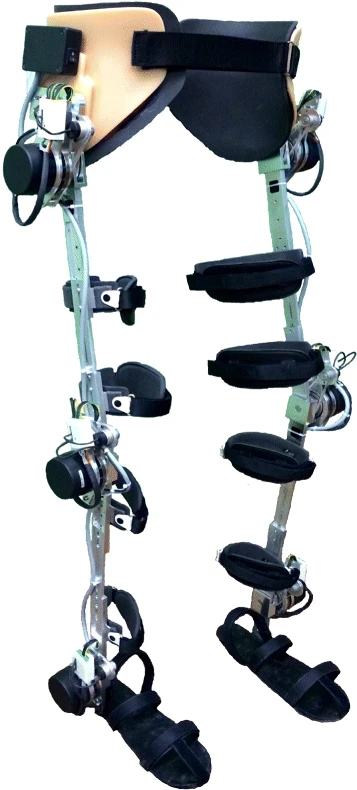
\includegraphics[width=0.3\linewidth]{Figures/Background/OtherExos/H2_Exo.png}
    \hspace{0.1\linewidth}
    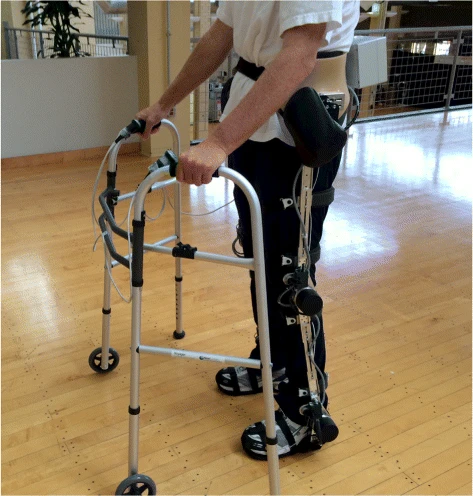
\includegraphics[width=0.5\linewidth]{Figures/Background/OtherExos/H2_ExoUse.png}
    \caption{The H2 Exoskeleton, with 6 powered joints and lithium polymer batteries \cite{ExoH2}}
    \label{fig:H2Exo}
\end{figure}

The H2 robotic exoskeleton is designed by the University of Houston to help stroke survivors with gait training and physical rehabilitation. It has 6 powerful DC motors (3 on each leg on the hip, knee, and ankle joint) geared down with harmonic gearboxes. Each motor is powered by its own local motor controller, with all electronics connected to a main controller via CAN bus. An assistive gait controller is used to apply torque when patients deviate from a planned gait pattern. The device itself was tested on 3 hemiparetic stroke patients, and was safe and effective throughout the 4 week testing period. The pilot clinical study demonstrated the "assist-as-needed" control system was able to benefit the stroke patients, and help them recover \cite{ExoH2}.

\subsection{ReWalk}
\begin{figure}[H]
    \centering
    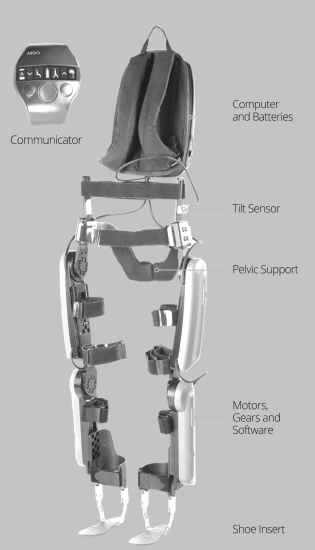
\includegraphics[width=0.4\linewidth]{Figures/Background/OtherExos/ReWalk.png}
    \caption{The Rewalk exoskeleton: an commercial exoskeleton with knee and hip powered joints \cite{ExoRewalk}.}
    \label{fig:RewalkExo}
\end{figure}

The {Rewalk\texttrademark} exoskeleton (Rewalk Robotics) is a commercial exoskeleton for lower-limb paralysis patients. Unlike most medical exoskeletons, Rewalk is designed for daily use - not just for rehabilitation in controlled environment. It consists of a lower-limb exoskeleton with powered rotary joints. The joints do not consider tibiofemoral joint trajectory, and have a static center of rotation. The system is all powered by a computer and batteries in a backpack worn by the user. Research by Talaty \textit{et. al} in \cite{ExoRewalk} demonstrated that assistive devices such as Rewalk are able to improve the walking capability of lower-limb paralysis patients with some practice. 

\subsection{EksoNR}
\begin{figure}[H]
    \centering
    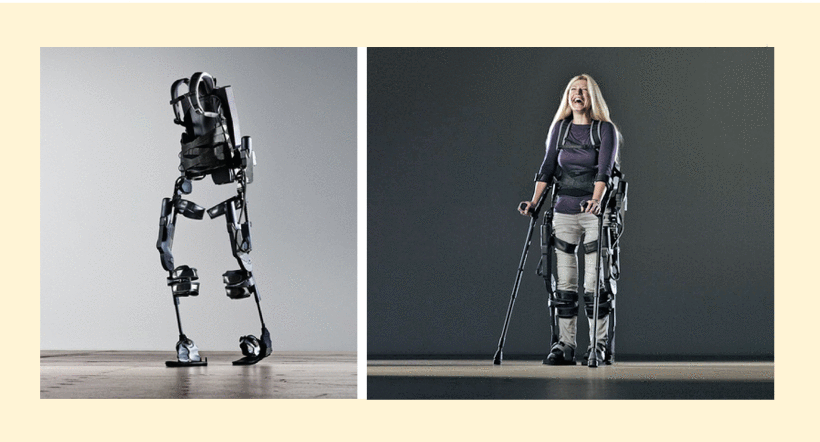
\includegraphics[width=0.9\linewidth]{Figures/Background/OtherExos/EKSO.png}
    \caption{The Ekso exoskeleton is a commercial rehabilitation system currently used in hospitals and rehabilitation centers.}
    \label{fig:EksoExo}
\end{figure}

The EksoNR exoskeleton (EksoBionics, Richmond California) is a commercial rehabilitation exoskeleton currently in clinical use since February 2012. EksoBionics - the company that manufactures this device - claims to be the only FDA-cleared exoskeleton for use with patients with acquired brain injury which has lead to paralysis. % TODO: Not true, see Indigo
It has similar functionality and features to the Rewalk; the hip, knee, and ankle joints are all actuated pin joints. The exoskeleton holds the control electronics and batteries in a backpack-like container, which doubles as a way to stabilize the patient's upper body during use \cite{ExoEksoNR}.

\subsection{Indigo}
\begin{figure}[H]
    \centering
    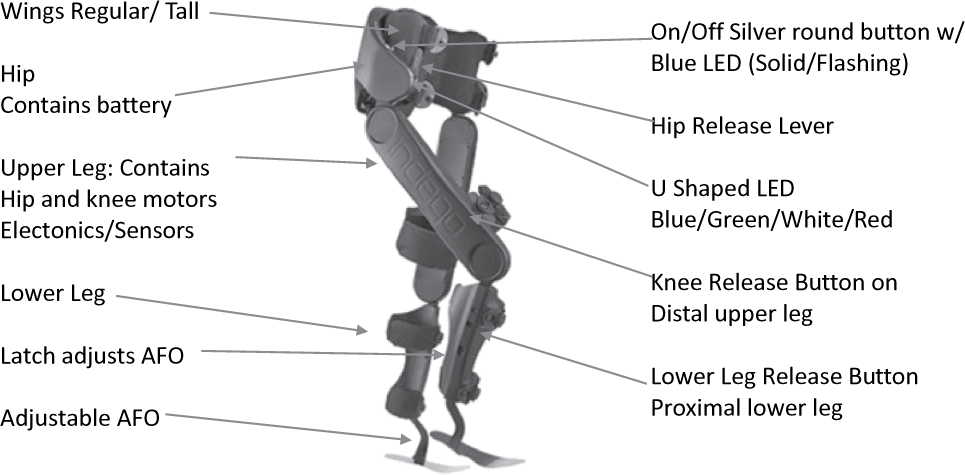
\includegraphics[width=0.9\linewidth]{Figures/Background/OtherExos/IndigoExo.png}
    \caption{The Indigo exoskeleton, which is used for clinical trials and paralysis rehabilitation \cite{IndigoClinicalStudy}}
    \label{fig:IndigoExo}
\end{figure}

The Indigo Therapy exoskeleton (Parker Hannifin, Macedonia, Ohio) is another commercial exoskeleton, specifically tailor made for spinal cord injuries and stroke patients. The device includes 4 motors - two hip and two knee actuators - and provide the support to move a patient for therapeutic and more recently personal use. According to Parker Hannifin, the Indigo exoskeleton has received FDA clearance for individuals with spinal cord injuries at levels between C7 and L5 to perform ambulatory functions for rehabilitation. Similar to most others, the batteries are held in and around the hip area, as seen in \autoref{fig:IndigoExo}.

% TODO: [maybe] If time, add these to the project
% \subsection{KINESIS}

% \subsection{HAL}